\chapter{Pràctica}
\label{cap:practica}

En aquest capítol es recullen exercicis resolts que permeten consolidar els conceptes principals de la teoria. Els primers exercicis treballen els nombres racionals des d'un punt de vista conceptual i procedimental. Els darrers exercicis mostren aplicacions dels nombres racionals a proporcions, escales, figures geomètriques i funcions de proporcionalitat.

\section{Construcció i representació dels nombres racionals}

\begin{exercici}[Fraccions com a classes]
	Decidiu si
	\[
		\frac{6}{10},\qquad \frac{9}{15},\qquad \frac{-3}{-5},\qquad \frac{12}{25}
	\]
	representen el mateix nombre racional.
\end{exercici}

\begin{solucio}
	Dues fraccions \(a/b\) i \(c/d\), amb denominadors no nuls, representen el mateix nombre racional si
	\[
		ad=bc.
	\]

	Primer comparem \(\frac{6}{10}\) i \(\frac{9}{15}\):
	\[
		6\cdot15=90
		\qquad\text{i}\qquad
		10\cdot9=90.
	\]
	Per tant,
	\[
		\frac{6}{10}=\frac{9}{15}.
	\]

	Ara comparem \(\frac{6}{10}\) i \(\frac{-3}{-5}\):
	\[
		6\cdot(-5)=-30
		\qquad\text{i}\qquad
		10\cdot(-3)=-30.
	\]
	Per tant,
	\[
		\frac{6}{10}=\frac{-3}{-5}.
	\]

	Finalment, comparem \(\frac{6}{10}\) i \(\frac{12}{25}\):
	\[
		6\cdot25=150
		\qquad\text{i}\qquad
		10\cdot12=120.
	\]
	Com que \(150\neq120\), tenim
	\[
		\frac{6}{10}\neq\frac{12}{25}.
	\]

	Així, les tres primeres fraccions representen el mateix nombre racional, però \(\frac{12}{25}\) representa un nombre racional diferent.
\end{solucio}

\begin{exercici}[Representants d'un nombre racional]
	Escriviu quatre representants diferents del nombre racional representat per
	\[
		-\frac{3}{4}.
	\]
\end{exercici}

\begin{solucio}
	Per obtenir fraccions equivalents, multipliquem el numerador i el denominador pel mateix enter no nul.

	Multiplicant per \(2\), \(3\), \(-1\) i \(-5\), obtenim
	\[
		-\frac{3}{4}
		=
		-\frac{6}{8}
		=
		-\frac{9}{12}
		=
		\frac{3}{-4}
		=
		\frac{15}{-20}.
	\]

	Per tant, quatre representants diferents del mateix nombre racional són
	\[
		-\frac{6}{8},\qquad
		-\frac{9}{12},\qquad
		\frac{3}{-4},\qquad
		\frac{15}{-20}.
	\]
\end{solucio}

\begin{exercici}[Els enters com a racionals]
	Escriviu els enters \(-3\), \(0\) i \(5\) com a nombres racionals. Doneu-ne dos representants diferents en cada cas.
\end{exercici}

\begin{solucio}
	Cada enter \(n\in\Z\) es pot identificar amb el racional representat per \(\frac{n}{1}\).

	Per tant,
	\[
		-3=\frac{-3}{1}=\frac{-6}{2},
	\]
	\[
		0=\frac{0}{1}=\frac{0}{7},
	\]
	i
	\[
		5=\frac{5}{1}=\frac{15}{3}.
	\]

	En tots els casos, el denominador ha de ser no nul.
\end{solucio}

\begin{exercici}[Fracció irreductible]
	Reduïu a fracció irreductible:
	\[
		\frac{-84}{126}.
	\]
\end{exercici}

\begin{solucio}
	Calculem el màxim comú divisor de \(84\) i \(126\):
	\[
		\mcd(84,126)=42.
	\]
	Dividim el numerador i el denominador per \(42\):
	\[
		\frac{-84}{126}
		=
		\frac{-84:42}{126:42}
		=
		-\frac{2}{3}.
	\]

	Per tant, la fracció irreductible equivalent és
	\[
		-\frac{2}{3}.
	\]
\end{solucio}

\begin{exercici}[Signe d'un racional]
	Escriviu amb denominador positiu i en forma irreductible:
	\[
		\frac{45}{-60}.
	\]
\end{exercici}

\begin{solucio}
	Primer passem el signe negatiu al numerador:
	\[
		\frac{45}{-60}
		=
		-\frac{45}{60}.
	\]
	Ara simplifiquem. Com que
	\[
		\mcd(45,60)=15,
	\]
	tindrem
	\[
		-\frac{45}{60}
		=
		-\frac{45:15}{60:15}
		=
		-\frac{3}{4}.
	\]

	Per tant,
	\[
		\frac{45}{-60}
		=
		-\frac{3}{4}.
	\]
\end{solucio}

\begin{exercici}[Ubicació sobre la recta numèrica amb el teorema de Tales]
	Expliqueu com es poden situar sobre la recta numèrica els nombres
	\[
		-\frac{2}{5}
		\qquad\text{i}\qquad
		\frac{7}{3}
	\]
	fent servir el teorema de Tales.
\end{exercici}

\begin{solucio}
	El teorema de Tales permet dividir un segment en parts iguals mitjançant rectes paral·leles. Aquesta construcció és especialment adequada per representar fraccions sobre la recta numèrica.

	Per situar \(-\frac{2}{5}\), dividim el segment que va de \(0\) a \(-1\) en cinc parts iguals. Com que el nombre és negatiu, ens desplacem cap a l'esquerra de l'origen i prenem la segona divisió.

	\begin{center}
	\begin{tikzpicture}[x=4cm,y=2.2cm]
		% Recta numerica
		\draw[->] (-1.18,0) -- (0.25,0);
		\foreach \x/\lab in {-1/{-1},0/{0}} {
			\draw (\x,0.035) -- (\x,-0.035);
			\node[below] at (\x,-0.035) {$\lab$};
		}

		% Construccio auxiliar de Tales
		\coordinate (O) at (0,0);
		\coordinate (A) at (-1,0);
		\coordinate (P1) at (0.15,0.24);
		\coordinate (P2) at (0.30,0.48);
		\coordinate (P3) at (0.45,0.72);
		\coordinate (P4) at (0.60,0.96);
		\coordinate (P5) at (0.75,1.20);
		\coordinate (X) at (-0.4,0);

		\draw (O) -- (P5);
		\foreach \P in {P1,P2,P3,P4,P5} {
			\fill[black] (\P) circle (0.8pt);
		}
		\draw (P5) -- (A);
		\draw (P2) -- (X);

		\fill[black] (O) circle (1.2pt);
		\fill[black] (A) circle (1.2pt);
		\fill[black] (X) circle (1.6pt);
		\node[above] at (X) {$-\frac{2}{5}$};

		\node[right] at (P5) {$5$ parts};
		\node[right] at (P2) {$2$ parts};
	\end{tikzpicture}

	\smallskip
	\textit{Construcció de \(-\frac{2}{5}\) dividint el segment \([0,-1]\) en cinc parts iguals mitjançant el teorema de Tales.}
	\end{center}

	Per situar \(\frac{7}{3}\), fem primer la divisió euclidiana
	\[
		7=3\cdot2+1.
	\]
	Així,
	\[
		\frac{7}{3}=2+\frac{1}{3}.
	\]
	Per tant, avancem fins al punt \(2\) i dividim el segment \([2,3]\) en tres parts iguals mitjançant el teorema de Tales. La primera divisió correspon al punt \(2+\frac{1}{3}=\frac{7}{3}\).

	\begin{center}
	\begin{tikzpicture}[x=2.2cm,y=2.2cm]
		% Recta numerica
		\draw[->] (-0.15,0) -- (3.35,0);
		\foreach \x/\lab in {0/{0},1/{1},2/{2},3/{3}} {
			\draw (\x,0.035) -- (\x,-0.035);
			\node[below] at (\x,-0.035) {$\lab$};
		}

		% Construccio auxiliar de Tales sobre [2,3]
		\coordinate (B) at (2,0);
		\coordinate (C) at (3,0);
		\coordinate (Q1) at (2.25,0.40);
		\coordinate (Q2) at (2.50,0.80);
		\coordinate (Q3) at (2.75,1.20);
		\coordinate (Y) at (2.333333,0);

		\draw (B) -- (Q3);
		\foreach \Q in {Q1,Q2,Q3} {
			\fill[black] (\Q) circle (0.8pt);
		}
		\draw (Q3) -- (C);
		\draw (Q1) -- (Y);

		\fill[black] (B) circle (1.2pt);
		\fill[black] (C) circle (1.2pt);
		\fill[black] (Y) circle (1.6pt);
		\node[above] at (Y) {$\frac{7}{3}$};

		\node[right] at (Q3) {$3$ parts};
		\node[right] at (Q1) {$1$ part};
	\end{tikzpicture}

	\smallskip
	\textit{Construcció de \(\frac{7}{3}=2+\frac{1}{3}\) dividint el segment \([2,3]\) en tres parts iguals mitjançant el teorema de Tales.}
	\end{center}
\end{solucio}

\section{Operacions amb nombres racionals}

\begin{exercici}[Addició i subtracció]
	Calculeu i simplifiqueu:
	\[
		\frac{3}{4}-\frac{5}{6}+\frac{2}{9}.
	\]
\end{exercici}

\begin{solucio}
	El mínim comú múltiple de \(4\), \(6\) i \(9\) és \(36\). Per tant,
	\[
		\frac{3}{4}-\frac{5}{6}+\frac{2}{9}
		=
		\frac{27}{36}-\frac{30}{36}+\frac{8}{36}
		=
		\frac{5}{36}.
	\]
\end{solucio}

\begin{exercici}[Multiplicació i divisió]
	Calculeu i simplifiqueu:
	\[
		\left(-\frac{5}{8}\right):\frac{15}{16}.
	\]
\end{exercici}

\begin{solucio}
	Dividir per un racional no nul és multiplicar pel seu invers:
	\[
		\left(-\frac{5}{8}\right):\frac{15}{16}
		=
		\left(-\frac{5}{8}\right)\cdot\frac{16}{15}.
	\]
	Simplifiquem abans de multiplicar:
	\[
		\left(-\frac{5}{8}\right)\cdot\frac{16}{15}
		=
		-\frac{5\cdot16}{8\cdot15}
		=
		-\frac{1\cdot2}{1\cdot3}
		=
		-\frac{2}{3}.
	\]

	Per tant,
	\[
		\left(-\frac{5}{8}\right):\frac{15}{16}
		=
		-\frac{2}{3}.
	\]
\end{solucio}

\begin{exercici}[Invers multiplicatiu]
	Trobeu l'invers multiplicatiu de
	\[
		\alpha=-\frac{7}{12}
	\]
	i comproveu que el producte és \(1\).
\end{exercici}

\begin{solucio}
	Com que \(\alpha\neq0\), el seu invers multiplicatiu és
	\[
		\alpha^{-1}=-\frac{12}{7}.
	\]
	En efecte,
	\[
		\left(-\frac{7}{12}\right)\left(-\frac{12}{7}\right)=\frac{84}{84}=1.
	\]
\end{solucio}

\section{Ordre, densitat i valor absolut}

\begin{exercici}[Ordre en \(\Q\)]
	Ordeneu de menor a major:
	\[
		-\frac{3}{4},
		\qquad
		-\frac{5}{6},
		\qquad
		\frac{2}{3},
		\qquad
		\frac{7}{10}.
	\]
\end{exercici}

\begin{solucio}
	Entre els nombres negatius, és més petit el que té valor absolut més gran:
	\[
		-\frac{5}{6}< -\frac{3}{4}.
	\]
	Entre els nombres positius, comparem en creu:
	\[
		\frac{2}{3}<\frac{7}{10}
		\quad\Longleftrightarrow\quad
		2\cdot10<3\cdot7.
	\]
	Com que \(20<21\), tenim
	\[
		\frac{2}{3}<\frac{7}{10}.
	\]
	Per tant,
	\[
		-\frac{5}{6}< -\frac{3}{4}<\frac{2}{3}<\frac{7}{10}.
	\]
\end{solucio}

\begin{exercici}[Densitat]
	Trobeu tres nombres racionals diferents entre \(\frac{1}{3}\) i \(\frac{1}{2}\).
\end{exercici}

\begin{solucio}
	Escrivim els dos nombres amb denominador comú:
	\[
		\frac{1}{3}=\frac{10}{30},
		\qquad
		\frac{1}{2}=\frac{15}{30}.
	\]
	Aleshores tres nombres racionals entre aquests dos són
	\[
		\frac{11}{30},
		\qquad
		\frac{12}{30}=\frac{2}{5},
		\qquad
		\frac{13}{30}.
	\]
\end{solucio}

\begin{exercici}[Valor absolut]
	Calculeu:
	\[
		\abs{-\frac{7}{5}},
		\qquad
		\abs{\frac{3}{8}},
		\qquad
		\abs{-\frac{11}{6}}-\abs{\frac{5}{3}}.
	\]
\end{exercici}

\begin{solucio}
	El valor absolut d'un nombre racional és la seva distància a \(0\) sobre la recta numèrica. Per tant,
	\[
		\abs{-\frac{7}{5}}=\frac{7}{5}
		\qquad\text{i}\qquad
		\abs{\frac{3}{8}}=\frac{3}{8}.
	\]
	Finalment,
	\[
		\abs{-\frac{11}{6}}-\abs{\frac{5}{3}}
		=
		\frac{11}{6}-\frac{5}{3}
		=
		\frac{11}{6}-\frac{10}{6}
		=
		\frac{1}{6}.
	\]
\end{solucio}

\section{Expressions decimals, potències i arrels}

\begin{exercici}[Expressió decimal finita]
	Decidiu si la fracció
	\[
		\frac{21}{56}
	\]
	té expressió decimal finita.
\end{exercici}

\begin{solucio}
	Primer reduïm la fracció a forma irreductible. Com que
	\[
		\mcd(21,56)=7,
	\]
	tindrem
	\[
		\frac{21}{56}
		=
		\frac{3}{8}.
	\]
	Ara observem que
	\[
		8=2^3.
	\]
	El denominador irreductible només té el factor primer \(2\). Per tant, la fracció té expressió decimal finita.

	De fet,
	\[
		\frac{3}{8}
		=
		\frac{375}{1000}
		=
		0{,}375.
	\]
\end{solucio}

\begin{exercici}[Expressió decimal periòdica]
	Decidiu si la fracció
	\[
		\frac{7}{12}
	\]
	té expressió decimal finita o periòdica.
\end{exercici}

\begin{solucio}
	La fracció \(\frac{7}{12}\) ja és irreductible, perquè
	\[
		\mcd(7,12)=1.
	\]
	El denominador és
	\[
		12=2^2\cdot3.
	\]
	Com que apareix el factor primer \(3\), que és diferent de \(2\) i de \(5\), la fracció no té expressió decimal finita.

	Per tant, té expressió decimal periòdica. En efecte,
	\[
		\frac{7}{12}=0{,}58\overline{3}.
	\]
\end{solucio}

\begin{exercici}[Fracció generatriu d'un decimal finit]
	Calculeu la fracció generatriu de
	\[
		3{,}075.
	\]
\end{exercici}

\begin{solucio}
	Com que hi ha tres xifres decimals, podem escriure
	\[
		3{,}075=\frac{3075}{1000}.
	\]
	Simplifiquem la fracció. Com que
	\[
		\mcd(3075,1000)=25,
	\]
	tindrem
	\[
		\frac{3075}{1000}
		=
		\frac{123}{40}.
	\]
	Per tant,
	\[
		3{,}075=\frac{123}{40}.
	\]
\end{solucio}

\begin{exercici}[Fracció generatriu d'un decimal periòdic]
	Calculeu la fracció generatriu de
	\[
		2{,}1\overline{37}.
	\]
\end{exercici}

\begin{solucio}
	Sigui
	\[
		x=2{,}1\overline{37}=2{,}1373737\ldots
	\]
	Hi ha una xifra no periòdica i dues xifres periòdiques. Multipliquem per \(10\) i per \(1000\):
	\[
		10x=21{,}373737\ldots,
		\qquad
		1000x=2137{,}373737\ldots
	\]
	Restant,
	\[
		1000x-10x=2137-21=2116.
	\]
	Així,
	\[
		990x=2116,
		\qquad
		x=\frac{2116}{990}=\frac{1058}{495}.
	\]
\end{solucio}

\begin{exercici}[Potències de racionals]
	Calculeu:
	\[
		\left(-\frac{2}{3}\right)^4
		\qquad\text{i}\qquad
		\left(-\frac{2}{3}\right)^5.
	\]
\end{exercici}

\begin{solucio}
	Quan l'exponent és parell, el resultat és positiu:
	\[
		\left(-\frac{2}{3}\right)^4
		=
		\frac{2^4}{3^4}
		=
		\frac{16}{81}.
	\]
	Quan l'exponent és senar, el resultat conserva el signe negatiu:
	\[
		\left(-\frac{2}{3}\right)^5
		=
		-\frac{2^5}{3^5}
		=
		-\frac{32}{243}.
	\]
\end{solucio}

\begin{exercici}[Propietats de les potències]
	Simplifiqueu l'expressió següent:
	\[
		\left(\frac{3}{5}\right)^2\cdot\left(\frac{3}{5}\right)^4:\left(\frac{3}{5}\right)^3.
	\]
\end{exercici}

\begin{solucio}
	Com que totes les potències tenen la mateixa base, podem sumar els exponents en la multiplicació i restar-los en la divisió:
	\[
		\left(\frac{3}{5}\right)^2\cdot\left(\frac{3}{5}\right)^4:
		\left(\frac{3}{5}\right)^3
		=
		\left(\frac{3}{5}\right)^{2+4-3}
		=
		\left(\frac{3}{5}\right)^3.
	\]
	Per tant,
	\[
		\left(\frac{3}{5}\right)^3
		=
		\frac{27}{125}.
	\]
\end{solucio}

\begin{exercici}[Arrels de racionals]
	Decidiu si les arrels següents són racionals:
	\[
		\sqrt{\frac{49}{81}},
		\qquad
		\sqrt{\frac{2}{9}}.
	\]
\end{exercici}

\begin{solucio}
	En el primer cas,
	\[
		\sqrt{\frac{49}{81}}
		=
		\frac{\sqrt{49}}{\sqrt{81}}
		=
		\frac{7}{9}.
	\]
	Per tant, és un nombre racional.

	En el segon cas,
	\[
		\sqrt{\frac{2}{9}}
		=
		\frac{\sqrt{2}}{3}.
	\]
	Com que \(\sqrt{2}\) no és racional, tampoc no ho és \(\frac{\sqrt{2}}{3}\).

	Per tant,
	\[
		\sqrt{\frac{49}{81}}\in\Q,
		\qquad
		\sqrt{\frac{2}{9}}\notin\Q.
	\]
\end{solucio}

\subsection{Operacions combinades amb fraccions, potències i arrels}

Un cop treballades les operacions bàsiques, les potències i les arrels, podem resoldre expressions on apareixen totes aquestes operacions combinades. Cal respectar l'ordre habitual de les operacions:
\[
\begin{array}{c}
	\text{parèntesis}
	\longrightarrow
	\text{potències i arrels} \\[2mm]
	\longrightarrow
	\text{multiplicacions i divisions}
	\longrightarrow
	\text{addicions i subtraccions}.
\end{array}
\]
També cal tenir cura amb els signes i simplificar sempre que sigui possible.

\begin{exercici}[Tres fraccions amb denominadors diferents]
	Calculeu:
	\[
		\frac{2}{3}+\frac{5}{6}-\frac{1}{4}.
	\]
\end{exercici}

\begin{solucio}
	Busquem un denominador comú. Com que
	\[
		\mcm(3,6,4)=12,
	\]
	tindrem
	\[
		\frac{2}{3}+\frac{5}{6}-\frac{1}{4}
		=
		\frac{8}{12}+\frac{10}{12}-\frac{3}{12}.
	\]
	Per tant,
	\[
		\frac{8}{12}+\frac{10}{12}-\frac{3}{12}
		=
		\frac{15}{12}
		=
		\frac{5}{4}.
	\]
\end{solucio}

\begin{exercici}[Parèntesis i multiplicació]
	Calculeu:
	\[
		\left(\frac{3}{4}-\frac{2}{3}\right)\cdot\frac{6}{5}+\frac{1}{2}.
	\]
\end{exercici}

\begin{solucio}
	Primer resolem el parèntesi:
	\[
		\frac{3}{4}-\frac{2}{3}
		=
		\frac{9}{12}-\frac{8}{12}
		=
		\frac{1}{12}.
	\]
	Així,
	\[
		\left(\frac{3}{4}-\frac{2}{3}\right)\cdot\frac{6}{5}+\frac{1}{2}
		=
		\frac{1}{12}\cdot\frac{6}{5}+\frac{1}{2}.
	\]
	Ara fem la multiplicació:
	\[
		\frac{1}{12}\cdot\frac{6}{5}
		=
		\frac{6}{60}
		=
		\frac{1}{10}.
	\]
	Finalment,
	\[
		\frac{1}{10}+\frac{1}{2}
		=
		\frac{1}{10}+\frac{5}{10}
		=
		\frac{6}{10}
		=
		\frac{3}{5}.
	\]
\end{solucio}

\begin{exercici}[Parèntesis i divisió]
	Calculeu:
	\[
		\left(\frac{5}{6}-\frac{1}{3}\right):\frac{2}{9}-\frac{3}{4}.
	\]
\end{exercici}

\begin{solucio}
	Primer resolem el parèntesi:
	\[
		\frac{5}{6}-\frac{1}{3}
		=
		\frac{5}{6}-\frac{2}{6}
		=
		\frac{3}{6}
		=
		\frac{1}{2}.
	\]
	Per tant,
	\[
		\left(\frac{5}{6}-\frac{1}{3}\right):\frac{2}{9}-\frac{3}{4}
		=
		\frac{1}{2}:\frac{2}{9}-\frac{3}{4}.
	\]
	Dividir per una fracció és multiplicar pel seu invers:
	\[
		\frac{1}{2}:\frac{2}{9}
		=
		\frac{1}{2}\cdot\frac{9}{2}
		=
		\frac{9}{4}.
	\]
	Ara restem:
	\[
		\frac{9}{4}-\frac{3}{4}
		=
		\frac{6}{4}
		=
		\frac{3}{2}.
	\]
\end{solucio}

\begin{exercici}[Prioritat de les operacions]
	Calculeu:
	\[
		\frac{3}{5}
		-
		\frac{7}{10}\cdot\frac{2}{3}
		+
		\frac{1}{4}:\frac{5}{8}.
	\]
\end{exercici}

\begin{solucio}
	Primer fem la multiplicació i la divisió:
	\[
		\frac{7}{10}\cdot\frac{2}{3}
		=
		\frac{14}{30}
		=
		\frac{7}{15},
	\]
	i
	\[
		\frac{1}{4}:\frac{5}{8}
		=
		\frac{1}{4}\cdot\frac{8}{5}
		=
		\frac{8}{20}
		=
		\frac{2}{5}.
	\]
	Per tant,
	\[
		\frac{3}{5}
		-
		\frac{7}{10}\cdot\frac{2}{3}
		+
		\frac{1}{4}:\frac{5}{8}
		=
		\frac{3}{5}-\frac{7}{15}+\frac{2}{5}.
	\]
	Ara reduïm a denominador comú:
	\[
		\frac{3}{5}-\frac{7}{15}+\frac{2}{5}
		=
		\frac{9}{15}-\frac{7}{15}+\frac{6}{15}
		=
		\frac{8}{15}.
	\]
\end{solucio}

\begin{exercici}[Potències i parèntesis]
	Calculeu:
	\[
		\left(-\frac{2}{3}\right)^2
		-
		\frac{5}{6}\left(\frac{3}{5}-\frac{1}{10}\right).
	\]
\end{exercici}

\begin{solucio}
	Primer calculem la potència:
	\[
		\left(-\frac{2}{3}\right)^2
		=
		\frac{4}{9}.
	\]
	Ara resolem el parèntesi:
	\[
		\frac{3}{5}-\frac{1}{10}
		=
		\frac{6}{10}-\frac{1}{10}
		=
		\frac{5}{10}
		=
		\frac{1}{2}.
	\]
	Per tant,
	\[
		\frac{5}{6}\left(\frac{3}{5}-\frac{1}{10}\right)
		=
		\frac{5}{6}\cdot\frac{1}{2}
		=
		\frac{5}{12}.
	\]
	Finalment,
	\[
		\frac{4}{9}-\frac{5}{12}
		=
		\frac{16}{36}-\frac{15}{36}
		=
		\frac{1}{36}.
	\]
\end{solucio}

\begin{exercici}[Potències, arrels i signes]
	Calculeu:
	\[
		\sqrt{\frac{25}{36}}
		+
		\sqrt[3]{-\frac{8}{27}}
		-
		\left(-\frac{1}{2}\right)^3.
	\]
\end{exercici}

\begin{solucio}
	Calculem cada terme per separat:
	\[
		\sqrt{\frac{25}{36}}
		=
		\frac{5}{6},
	\]
	ja que l'arrel quadrada principal és no negativa.

	També tenim
	\[
		\sqrt[3]{-\frac{8}{27}}
		=
		-\frac{2}{3},
	\]
	perquè
	\[
		\left(-\frac{2}{3}\right)^3
		=
		-\frac{8}{27}.
	\]
	Finalment,
	\[
		\left(-\frac{1}{2}\right)^3
		=
		-\frac{1}{8}.
	\]
	Així,
	\[
		\sqrt{\frac{25}{36}}
		+
		\sqrt[3]{-\frac{8}{27}}
		-
		\left(-\frac{1}{2}\right)^3
		=
		\frac{5}{6}-\frac{2}{3}-\left(-\frac{1}{8}\right).
	\]
	Per tant,
	\[
		\frac{5}{6}-\frac{2}{3}+\frac{1}{8}
		=
		\frac{5}{6}-\frac{4}{6}+\frac{1}{8}
		=
		\frac{1}{6}+\frac{1}{8}
		=
		\frac{4}{24}+\frac{3}{24}
		=
		\frac{7}{24}.
	\]
\end{solucio}

\section{Raons, proporcions i proporcionalitat aritmètica}

\begin{exercici}[Raó entre dues quantitats]
	En una classe hi ha \(18\) alumnes que estudien francès i \(12\) alumnes que estudien alemany. Calculeu la raó entre el nombre d'alumnes que estudien francès i el nombre d'alumnes que estudien alemany. Interpreteu-ne el resultat.
\end{exercici}

\begin{solucio}
	La raó demanada és
	\[
		\frac{18}{12}=\frac{3}{2}.
	\]
	Això vol dir que, per cada \(2\) alumnes que estudien alemany, n'hi ha \(3\) que estudien francès.
\end{solucio}

\begin{exercici}[Proporcions]
	Decidiu si l'expressió següent és una proporció:
	\[
		\frac{8}{12}=\frac{10}{15}.
	\]
\end{exercici}

\begin{solucio}
	Comprovem el producte dels mitjans i el producte dels extrems:
	\[
		12\cdot10=120
		\qquad\text{i}\qquad
		8\cdot15=120.
	\]
	Com que coincideixen,
	\[
		\frac{8}{12}=\frac{10}{15}
	\]
	és una proporció.
\end{solucio}

\begin{exercici}[Propietats de les proporcions]
	A partir de la proporció
	\[
		\frac{6}{8}=\frac{9}{12},
	\]
	escriviu la proporció inversa, la proporció alternada i la proporció que s'obté sumant els termes de cada raó.
\end{exercici}

\begin{solucio}
	La proporció inversa és
	\[
		\frac{8}{6}=\frac{12}{9}.
	\]

	La proporció alternada és
	\[
		\frac{6}{9}=\frac{8}{12}.
	\]

	Sumant els termes de cada raó, obtenim
	\[
		\frac{6+8}{8}=\frac{9+12}{12},
	\]
	és a dir,
	\[
		\frac{14}{8}=\frac{21}{12}.
	\]
\end{solucio}

\begin{exercici}[Tercera proporcional]
	Trobeu la tercera proporcional de \(2\) i \(6\).
\end{exercici}

\begin{solucio}
	Busquem \(x\in\Q\) tal que
	\[
		\frac{2}{6}=\frac{6}{x}.
	\]
	Pel producte dels mitjans i dels extrems,
	\[
		2x=36.
	\]
	Per tant,
	\[
		x=18.
	\]
	Així, la tercera proporcional de \(2\) i \(6\) és \(18\).
\end{solucio}

\begin{exercici}[Quarta proporcional]
	Trobeu la quarta proporcional de \(3\), \(5\) i \(9\).
\end{exercici}

\begin{solucio}
	Busquem \(x\in\Q\) tal que
	\[
		\frac{3}{5}=\frac{9}{x}.
	\]
	Pel producte dels mitjans i dels extrems,
	\[
		3x=45.
	\]
	Per tant,
	\[
		x=15.
	\]
	Així, la quarta proporcional de \(3\), \(5\) i \(9\) és \(15\).
\end{solucio}

\begin{exercici}[Mitjana proporcional]
	Trobeu la mitjana proporcional positiva de \(4\) i \(9\).
\end{exercici}

\begin{solucio}
	Busquem \(x\in\Q\), amb \(x>0\), tal que
	\[
		\frac{4}{x}=\frac{x}{9}.
	\]
	Pel producte dels mitjans i dels extrems,
	\[
		x^2=36.
	\]
	Com que \(x>0\), obtenim
	\[
		x=6.
	\]
	Així, la mitjana proporcional positiva de \(4\) i \(9\) és \(6\).
\end{solucio}


\begin{exercici}[Identificació d'una relació entre magnituds]
	Observeu la taula següent, que relaciona dues magnituds \(x\) i \(y\):
	\[
	\begin{array}{c|cccc}
		x & 2 & 5 & 8 & 11 \\
		\hline
		y & 6 & 15 & 24 & ?
	\end{array}
	\]
	Decidiu quin tipus de relació hi ha entre les dues magnituds i calculeu el valor que falta.
\end{exercici}

\begin{solucio}
	No hem d'aplicar una regla mecànicament: primer cal decidir quina relació hi ha entre les magnituds.

	Comprovem si el quocient \(y/x\) és constant:
	\[
		\frac{6}{2}=3,
		\qquad
		\frac{15}{5}=3,
		\qquad
		\frac{24}{8}=3.
	\]
	Com que el quocient és constant, les dues magnituds són directament proporcionals.

	Per tant,
	\[
		\frac{y}{x}=3,
	\]
	i, quan \(x=11\), tenim
	\[
		y=3\cdot 11=33.
	\]
	El valor que falta és \(33\).
\end{solucio}

\begin{exercici}[Identificació d'una relació entre magnituds]
	Observeu la taula següent, que relaciona dues magnituds \(x\) i \(y\):
	\[
	\begin{array}{c|cccc}
		x & 2 & 3 & 6 & 9 \\
		\hline
		y & 18 & 12 & 6 & ?
	\end{array}
	\]
	Decidiu quin tipus de relació hi ha entre les dues magnituds i calculeu el valor que falta.
\end{exercici}

\begin{solucio}
	Primer comprovem si el quocient \(y/x\) és constant:
	\[
		\frac{18}{2}=9,
		\qquad
		\frac{12}{3}=4,
		\qquad
		\frac{6}{6}=1.
	\]
	El quocient no és constant, de manera que no és una relació de proporcionalitat directa.

	Ara comprovem el producte \(xy\):
	\[
		2\cdot 18=36,
		\qquad
		3\cdot 12=36,
		\qquad
		6\cdot 6=36.
	\]
	Com que el producte és constant, les dues magnituds són inversament proporcionals.

	Per tant,
	\[
		xy=36.
	\]
	Quan \(x=9\), tenim
	\[
		9y=36,
		\qquad
		y=4.
	\]
	El valor que falta és \(4\).
\end{solucio}

\section{Aplicacions a problemes de la vida real}

Els nombres racionals i les relacions de proporcionalitat apareixen en moltes situacions quotidianes: consum, preus, percentatges, repartiments, mescles, escales i temps de treball. En aquests problemes, l'enunciat no sempre indica si la relació és directa o inversa. Per això, abans de calcular, cal identificar les magnituds que intervenen i raonar com varia una quan varia l'altra.

\begin{exercici}[Recepta per a més racions]
	Una recepta utilitza \(250\) g de farina per preparar \(4\) racions. Quanta farina caldrà per preparar \(10\) racions, mantenint la mateixa recepta?
\end{exercici}

\begin{solucio}
	Primer identifiquem les magnituds: nombre de racions i quantitat de farina.

	Si preparem més racions mantenint la mateixa recepta, cal més farina en la mateixa proporció. Per tant, són magnituds directament proporcionals.

	Plantegem la proporció:
	\[
		\frac{250}{4}=\frac{x}{10}.
	\]
	Pel producte dels mitjans i dels extrems,
	\[
		4x=2500,
		\qquad
		x=625.
	\]
	Calen \(625\) g de farina.
\end{solucio}

\begin{exercici}[Mateixa feina amb més persones]
	Tres treballadors poden acabar una feina en \(8\) hores. Quant temps necessitaran \(6\) treballadors per fer la mateixa feina, si tots treballen al mateix ritme?
\end{exercici}

\begin{solucio}
	Les magnituds són el nombre de treballadors i el temps necessari.

	Com que la feina total és la mateixa, si hi treballen més persones, el temps disminueix. Per tant, les magnituds són inversament proporcionals.

	En una relació inversa, el producte es manté constant:
	\[
		3\cdot 8=6\cdot x.
	\]
	Així,
	\[
		24=6x,
		\qquad
		x=4.
	\]
	Per tant, \(6\) treballadors necessitaran \(4\) hores.
\end{solucio}

\begin{exercici}[Producció amb dues magnituds variables]
	Cinc màquines produeixen \(480\) peces treballant \(4\) dies a raó de \(6\) hores diàries. Quantes peces produiran \(8\) màquines treballant \(5\) dies a raó de \(7\) hores diàries, si totes les màquines tenen el mateix rendiment?
\end{exercici}

\begin{solucio}
	La producció depèn de tres magnituds: nombre de màquines, nombre de dies i hores de treball per dia.

	Si augmenta el nombre de màquines, augmenta la producció. Si augmenta el nombre de dies, també augmenta la producció. I si augmenten les hores diàries, també augmenta la producció. Per tant, la producció és directament proporcional a cadascuna d'aquestes magnituds.

	Passem de \(5\) màquines a \(8\) màquines: el factor és
	\[
		\frac{8}{5}.
	\]
	Passem de \(4\) dies a \(5\) dies: el factor és
	\[
		\frac{5}{4}.
	\]
	Passem de \(6\) hores diàries a \(7\) hores diàries: el factor és
	\[
		\frac{7}{6}.
	\]
	Per tant,
	\[
		x=480\cdot\frac{8}{5}\cdot\frac{5}{4}\cdot\frac{7}{6}.
	\]
	Simplificant,
	\[
		x=1120.
	\]
	Així, produiran \(1120\) peces.
\end{solucio}

\begin{exercici}[Percentatges]
	Una jaqueta costa \(80\) euros i té un descompte del \(15\%\). Quin és el preu final?
\end{exercici}

\begin{solucio}
	Calculem primer el descompte:
	\[
		15\%\text{ de }80
		=
		\frac{15}{100}\cdot80
		=
		12.
	\]
	El descompte és de \(12\) euros. Per tant, el preu final és
	\[
		80-12=68.
	\]

	La jaqueta costa finalment \(68\) euros.
\end{solucio}

\begin{exercici}[Increment percentual]
	El preu d'un producte era de \(50\) euros i ha augmentat un \(8\%\). Quin és el nou preu?
\end{exercici}

\begin{solucio}
	Calculem l'increment:
	\[
		8\%\text{ de }50
		=
		\frac{8}{100}\cdot50
		=
		4.
	\]
	El preu augmenta \(4\) euros. Per tant, el nou preu és
	\[
		50+4=54.
	\]

	El nou preu és \(54\) euros.
\end{solucio}

\begin{exercici}[Comparació de preus]
	En un supermercat, un paquet de \(750\) g d'arròs costa \(2{,}85\) euros, i un paquet d'\(1{,}2\) kg costa \(4{,}20\) euros. Quin paquet té millor preu per quilogram?
\end{exercici}

\begin{solucio}
	Per poder comparar els dos paquets, hem de calcular el preu d'una mateixa quantitat, per exemple el preu per quilogram.

	El primer paquet té \(750\) g, és a dir,
	\[
		750\text{ g}=0{,}75\text{ kg}.
	\]
	Per tant, el seu preu per quilogram és
	\[
		\frac{2{,}85}{0{,}75}=3{,}80.
	\]
	Així, el primer paquet costa \(3{,}80\) euros per quilogram.

	Per al segon paquet, tenim
	\[
		\frac{4{,}20}{1{,}2}=3{,}50.
	\]
	Així, el segon paquet costa \(3{,}50\) euros per quilogram.

	Com que
	\[
		3{,}50<3{,}80,
	\]
	el paquet d'\(1{,}2\) kg té millor preu per quilogram.
\end{solucio}

\begin{exercici}[Preparació d'una mescla]
	Un producte concentrat s'ha de barrejar amb aigua en la raó
	\[
		1:4,
	\]
	és a dir, una part de producte concentrat per cada quatre parts d'aigua. Quina quantitat de producte concentrat i quina quantitat d'aigua calen per preparar \(2{,}5\) litres de mescla?
\end{exercici}

\begin{solucio}
	La raó \(1:4\) indica que, de cada \(5\) parts de mescla, \(1\) part és producte concentrat i \(4\) parts són aigua.

	Per tant, la quantitat de producte concentrat és
	\[
		\frac{1}{5}\cdot2{,}5=0{,}5.
	\]
	La quantitat d'aigua és
	\[
		\frac{4}{5}\cdot2{,}5=2.
	\]

	Així, calen \(0{,}5\) litres de producte concentrat i \(2\) litres d'aigua.
\end{solucio}

\begin{exercici}[Velocitat i temps]
	Un cotxe fa un trajecte a una velocitat constant de \(90\) km/h i triga \(2\) hores. Quant temps trigaria a fer el mateix trajecte a \(120\) km/h, si manté aquesta nova velocitat constant?
\end{exercici}

\begin{solucio}
	Les magnituds són la velocitat i el temps. Com que el trajecte és el mateix, si augmenta la velocitat, disminueix el temps. Per tant, la relació és inversa.

	Primer calculem la distància del trajecte:
	\[
		90\cdot2=180.
	\]
	Per tant, el trajecte fa \(180\) km.

	Si la velocitat és de \(120\) km/h, el temps necessari és
	\[
		\frac{180}{120}=\frac{3}{2}=1{,}5.
	\]

	Així, trigaria \(1{,}5\) hores, és a dir, \(1\) hora i \(30\) minuts.
\end{solucio}

\begin{exercici}[Repartiment segons aportacions]
	Tres persones han participat en un projecte durant \(2\), \(3\) i \(5\) hores, respectivament. Es vol repartir una gratificació total de \(600\) euros tenint en compte el temps de participació de cadascuna. Quina quantitat ha de rebre cada persona?
\end{exercici}

\begin{solucio}
	Cal interpretar el criteri de repartiment. Com que es vol tenir en compte el temps de participació, qui ha dedicat més hores ha de rebre una part més gran. Per tant, el repartiment ha de ser proporcional a les hores dedicades.

	Si les parts són proporcionals a \(2\), \(3\) i \(5\), les podem escriure com
	\[
		2k,	\quad 3k,	\quad 5k.
	\]
	Com que la suma total és \(600\), tenim
	\[
		2k+3k+5k=600.
	\]
	Per tant,
	\[
		10k=600,
		\qquad
		k=60.
	\]
	Les tres parts són
	\[
		2k=120,	\qquad 3k=180,	\qquad 5k=300.
	\]
	Per tant, el repartiment és
	\[
		120\text{ euros},\qquad 180\text{ euros},\qquad 300\text{ euros}.
	\]
\end{solucio}

\begin{exercici}[Repartiment segons rapidesa]
	Tres equips han fet la mateixa tasca en \(2\), \(3\) i \(6\) hores, respectivament. Es vol repartir una prima total de \(780\) euros segons la rapidesa amb què han acabat la tasca. Quina quantitat ha de rebre cada equip?
\end{exercici}

\begin{solucio}
	Aquí cal pensar el criteri de repartiment. Tots els equips han fet la mateixa tasca, però no han trigat el mateix temps. Ser més ràpid vol dir trigar menys temps. Per tant, la rapidesa és proporcional a l'invers del temps.

	Així, el repartiment s'ha de fer proporcionalment a
	\[
		\frac{1}{2},\quad \frac{1}{3},\quad \frac{1}{6}.
	\]
	La suma d'aquests inversos és
	\[
		\frac{1}{2}+\frac{1}{3}+\frac{1}{6}
		=
		\frac{3}{6}+\frac{2}{6}+\frac{1}{6}
		=
		1.
	\]
	Per tant, les parts són
	\[
	\begin{aligned}
		x&=\frac{1}{2}\cdot780=390,\\
		y&=\frac{1}{3}\cdot780=260,\\
		z&=\frac{1}{6}\cdot780=130.
	\end{aligned}
	\]
	Així, el repartiment és
	\[
		390\text{ euros},\qquad 260\text{ euros},\qquad 130\text{ euros}.
	\]
\end{solucio}

\section{Proporcionalitat geomètrica i funcions de proporcionalitat}

\begin{exercici}[Escales]
	En un plànol a escala \(1:200\), una habitació fa \(4\) cm de llarg. Quina és la longitud real de l'habitació?
\end{exercici}

\begin{solucio}
	L'escala \(1:200\) vol dir que
	\[
		1\text{ cm en el plànol}=200\text{ cm en la realitat}.
	\]
	Per tant,
	\[
		4\text{ cm en el plànol}=4\cdot200=800\text{ cm en la realitat}.
	\]
	Com que
	\[
		800\text{ cm}=8\text{ m},
	\]
	la longitud real de l'habitació és \(8\) m.
\end{solucio}

\begin{exercici}[Proporcionalitat geomètrica]
	Dos triangles semblants tenen costats corresponents de longituds \(6\) cm i \(9\) cm. Si un altre costat del primer triangle fa \(10\) cm, quant fa el costat corresponent del segon triangle?
\end{exercici}

\begin{solucio}
	Com que els triangles són semblants, els costats corresponents són proporcionals. El factor d'escala del primer triangle al segon és
	\[
		k=\frac{9}{6}=\frac{3}{2}.
	\]
	Per tant, el costat corresponent al costat de \(10\) cm mesura
	\[
		10\cdot\frac{3}{2}=15.
	\]

	Així, el costat corresponent del segon triangle fa \(15\) cm.
\end{solucio}

\begin{exercici}[Teorema de Tales]
	Dues rectes secants són tallades per rectes paral·leles. En una de les secants es determinen dos segments de \(4\) cm i \(6\) cm. En l'altra secant, el segment corresponent al de \(4\) cm fa \(10\) cm. Quant fa el segment corresponent al de \(6\) cm?
\end{exercici}

\begin{solucio}
	Pel teorema de Tales, els segments corresponents són proporcionals. Si anomenem \(x\) el segment desconegut, tenim
	\[
		\frac{4}{6}
		=
		\frac{10}{x}.
	\]
	Pel producte dels mitjans i dels extrems,
	\[
		4x=60.
	\]
	Per tant,
	\[
		x=15.
	\]

	El segment desconegut fa \(15\) cm.
\end{solucio}

\begin{exercici}[Funció de proporcionalitat directa]
	El preu d'un quilogram de fruita és de \(2{,}40\) euros. Escriviu la funció que dona el preu total \(y\) en funció dels quilograms comprats \(x\), i calculeu el preu de \(3{,}5\) kg.
\end{exercici}

\begin{solucio}
	El preu total és directament proporcional al nombre de quilograms comprats. La constant de proporcionalitat és
	\[
		k=2{,}40.
	\]
	Per tant, la funció és
	\[
		y=2{,}40x.
	\]
	Si comprem \(3{,}5\) kg, aleshores
	\[
		y=2{,}40\cdot3{,}5=8{,}40.
	\]

	El preu de \(3{,}5\) kg és \(8{,}40\) euros.
\end{solucio}

\begin{exercici}[Taula de valors d'una funció de proporcionalitat directa]
	Considereu la funció
	\[
		f(x)=2x.
	\]
	Calculeu \(f(-2)\), \(f(-1)\), \(f(0)\), \(f(1)\) i \(f(2)\), i indiqueu els punts corresponents.
\end{exercici}

\begin{solucio}
	Calculem els valors demanats:
	\[
	\begin{array}{c|ccccc}
		x & -2 & -1 & 0 & 1 & 2 \\
		\hline
		f(x)=2x & -4 & -2 & 0 & 2 & 4
	\end{array}
	\]
	Els punts corresponents són
	\[
		(-2,-4),\quad (-1,-2),\quad (0,0),\quad (1,2),\quad (2,4).
	\]
	Representem aquests punts en el pla cartesià:

	\begin{center}
	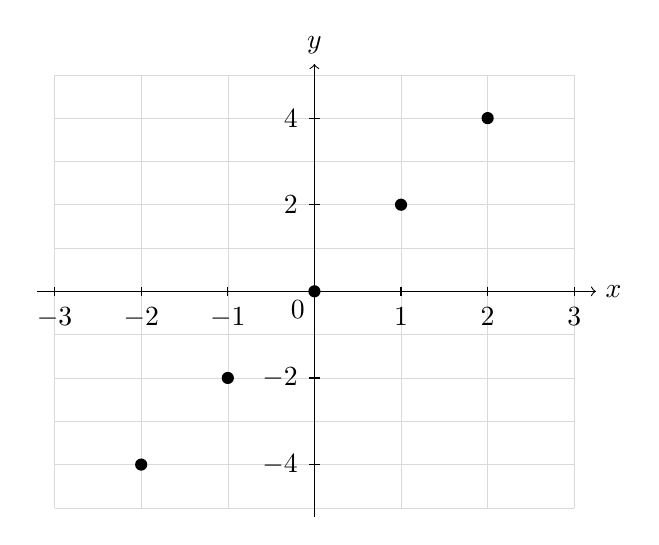
\begin{tikzpicture}[x=1.1cm,y=0.55cm]
		\draw[step=1, very thin, gray!30] (-3,-5) grid (3,5);
		\draw[->] (-3.2,0) -- (3.25,0) node[right] {$x$};
		\draw[->] (0,-5.2) -- (0,5.25) node[above] {$y$};
		\foreach \x in {-3,-2,-1,1,2,3} {
			\draw (\x,0.10) -- (\x,-0.10);
			\node[below] at (\x,-0.15) {$\x$};
		}
		\foreach \y in {-4,-2,2,4} {
			\draw (0.06,\y) -- (-0.06,\y);
			\node[left] at (-0.08,\y) {$\y$};
		}
		\node[below left] at (0,0) {$0$};
		\fill[black] (-2,-4) circle (2.2pt);
		\fill[black] (-1,-2) circle (2.2pt);
		\fill[black] (0,0) circle (2.2pt);
		\fill[black] (1,2) circle (2.2pt);
		\fill[black] (2,4) circle (2.2pt);
	\end{tikzpicture}

	\smallskip
	\textit{Punts de la funció de proporcionalitat directa $f(x)=2x$.}
	\end{center}

	Aquests punts estan alineats. Si es considerés la funció sobre \(\R\), la gràfica seria una recta que passa per l'origen.
\end{solucio}

\begin{exercici}[Funció de proporcionalitat inversa]
	Una feina requereix \(48\) hores de treball total. Si hi treballen \(x\) persones al mateix ritme, el temps necessari és \(y\). Escriviu la funció que relaciona \(x\) i \(y\), i calculeu el temps necessari si hi treballen \(6\) persones.
\end{exercici}

\begin{solucio}
	Com que el nombre de persones i el temps són inversament proporcionals, el producte es manté constant:
	\[
		xy=48.
	\]
	Per tant,
	\[
		y=\frac{48}{x}.
	\]
	Si hi treballen \(6\) persones, aleshores
	\[
		y=\frac{48}{6}=8.
	\]

	Per tant, \(6\) persones necessitaran \(8\) hores.
\end{solucio}

\begin{exercici}[Taula de valors d'una funció de proporcionalitat inversa]
	Considereu la funció
	\[
		f(x)=\frac{6}{x}.
	\]
	Calculeu-ne alguns valors racionals i indiqueu els punts corresponents.
\end{exercici}

\begin{solucio}
	La funció no està definida en \(x=0\). Calculem alguns valors:
	\[
	\begin{array}{c|cccccccc}
		x & -6 & -3 & -2 & -1 & 1 & 2 & 3 & 6 \\
		\hline
		f(x)=\frac{6}{x} & -1 & -2 & -3 & -6 & 6 & 3 & 2 & 1
	\end{array}
	\]
	Els punts corresponents són
	\[
		(-6,-1),\quad (-3,-2),\quad (-2,-3),\quad (-1,-6),
	\]
	\[
		(1,6),\quad (2,3),\quad (3,2),\quad (6,1).
	\]
	Representem aquests punts en el pla cartesià:

	\begin{center}
	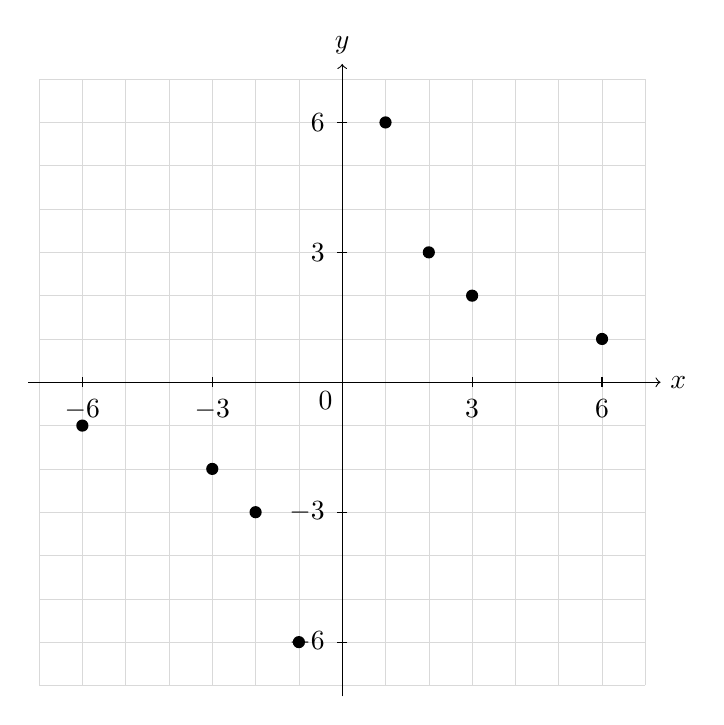
\begin{tikzpicture}[x=0.55cm,y=0.55cm]
		\draw[step=1, very thin, gray!30] (-7,-7) grid (7,7);
		\draw[->] (-7.25,0) -- (7.35,0) node[right] {$x$};
		\draw[->] (0,-7.25) -- (0,7.35) node[above] {$y$};
		\foreach \x in {-6,-3,3,6} {
			\draw (\x,0.12) -- (\x,-0.12);
			\node[below] at (\x,-0.18) {$\x$};
		}
		\foreach \y in {-6,-3,3,6} {
			\draw (0.12,\y) -- (-0.12,\y);
			\node[left] at (-0.18,\y) {$\y$};
		}
		\node[below left] at (0,0) {$0$};
		\fill[black] (-6,-1) circle (2.2pt);
		\fill[black] (-3,-2) circle (2.2pt);
		\fill[black] (-2,-3) circle (2.2pt);
		\fill[black] (-1,-6) circle (2.2pt);
		\fill[black] (1,6) circle (2.2pt);
		\fill[black] (2,3) circle (2.2pt);
		\fill[black] (3,2) circle (2.2pt);
		\fill[black] (6,1) circle (2.2pt);
	\end{tikzpicture}

	\smallskip
	\textit{Punts de la funció de proporcionalitat inversa $f(x)=\frac{6}{x}$.}
	\end{center}

	Aquests punts no estan alineats. Si es considerés la funció sobre \(\R\), la gràfica seria una hipèrbola.
\end{solucio}
